\subsubsubsubsection{Stretch}
\begin{figure}[h]
\centering
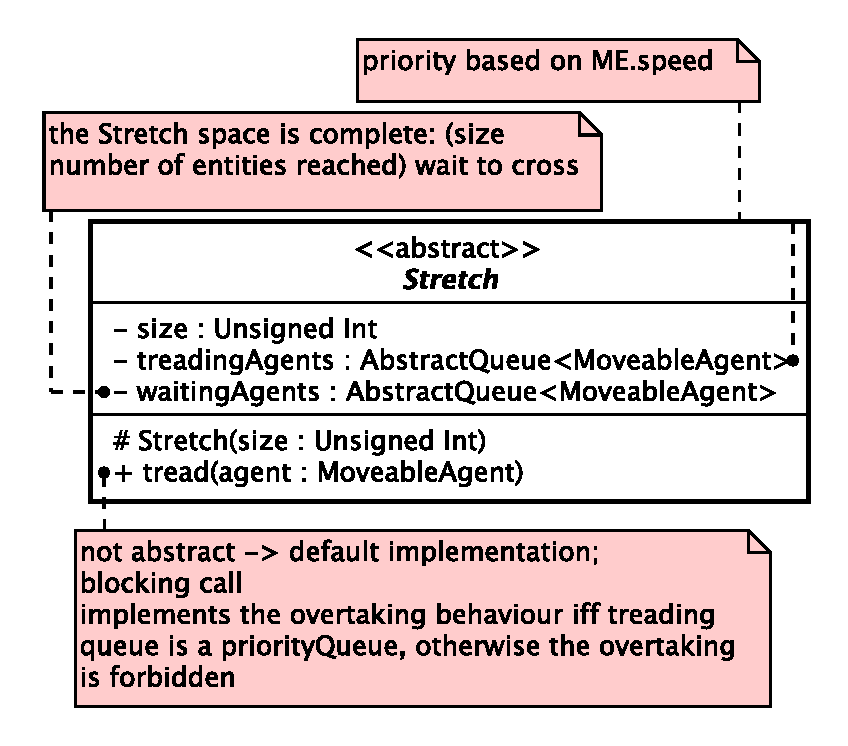
\includegraphics[scale=0.6,keepaspectratio]{images/solution/app/backend/stretch.eps}
\caption{\pReactiveComponentStretch::Stretch}
\label{fig:sd-app-stretch}
\end{figure}
\FloatBarrier
\begin{itemize}
  \item \textbf{\descr} \\
    It represents a stretch entity. It is a protected object.
  \item \textbf{\attrs}
  \begin{itemize}
    \item \texttt{size: Unsigned Int} \\
The size of the stretch/treading queue.
    \item \texttt{treadingAgents: AbstractQueue<MoveableAgent>} \\
The queue of urban actors which are treading the stretch. If the concrete type
is PriorityQueue then the stretch allows the overtaking between the urban actors.
This is implemented through a priority queue ordered by decreasing speed.
    \item \texttt{waitingAgents: AbstractQueue<MoveableAgent>} \\
The queue of urban actors which are waiting to tread the stretch. 
  \end{itemize}
  \item \textbf{\ops}
  \begin{itemize}
    \item[\#] \texttt{Stretch(size: Unsigned Int)} \\
Creates a stretch object with a specific size.
    \item[+] \texttt{tread(agent: MoveableAgent)} \\
Implements the stretch treading. The current speed of the urban actor
is calculated first, then the entity is placed in a treading queue which has a  
timeout. When this timeout expires, the queue is flushed and the entity can
proceed along their route.
  \end{itemize}
\end{itemize}
